% Remember to input this to the presentative tex file before compiling.
\section{Results and Discussion}
\subsection{Results}
\begin{frame}
\begin{columns}
   
\begin{column}{0.7\textwidth}
    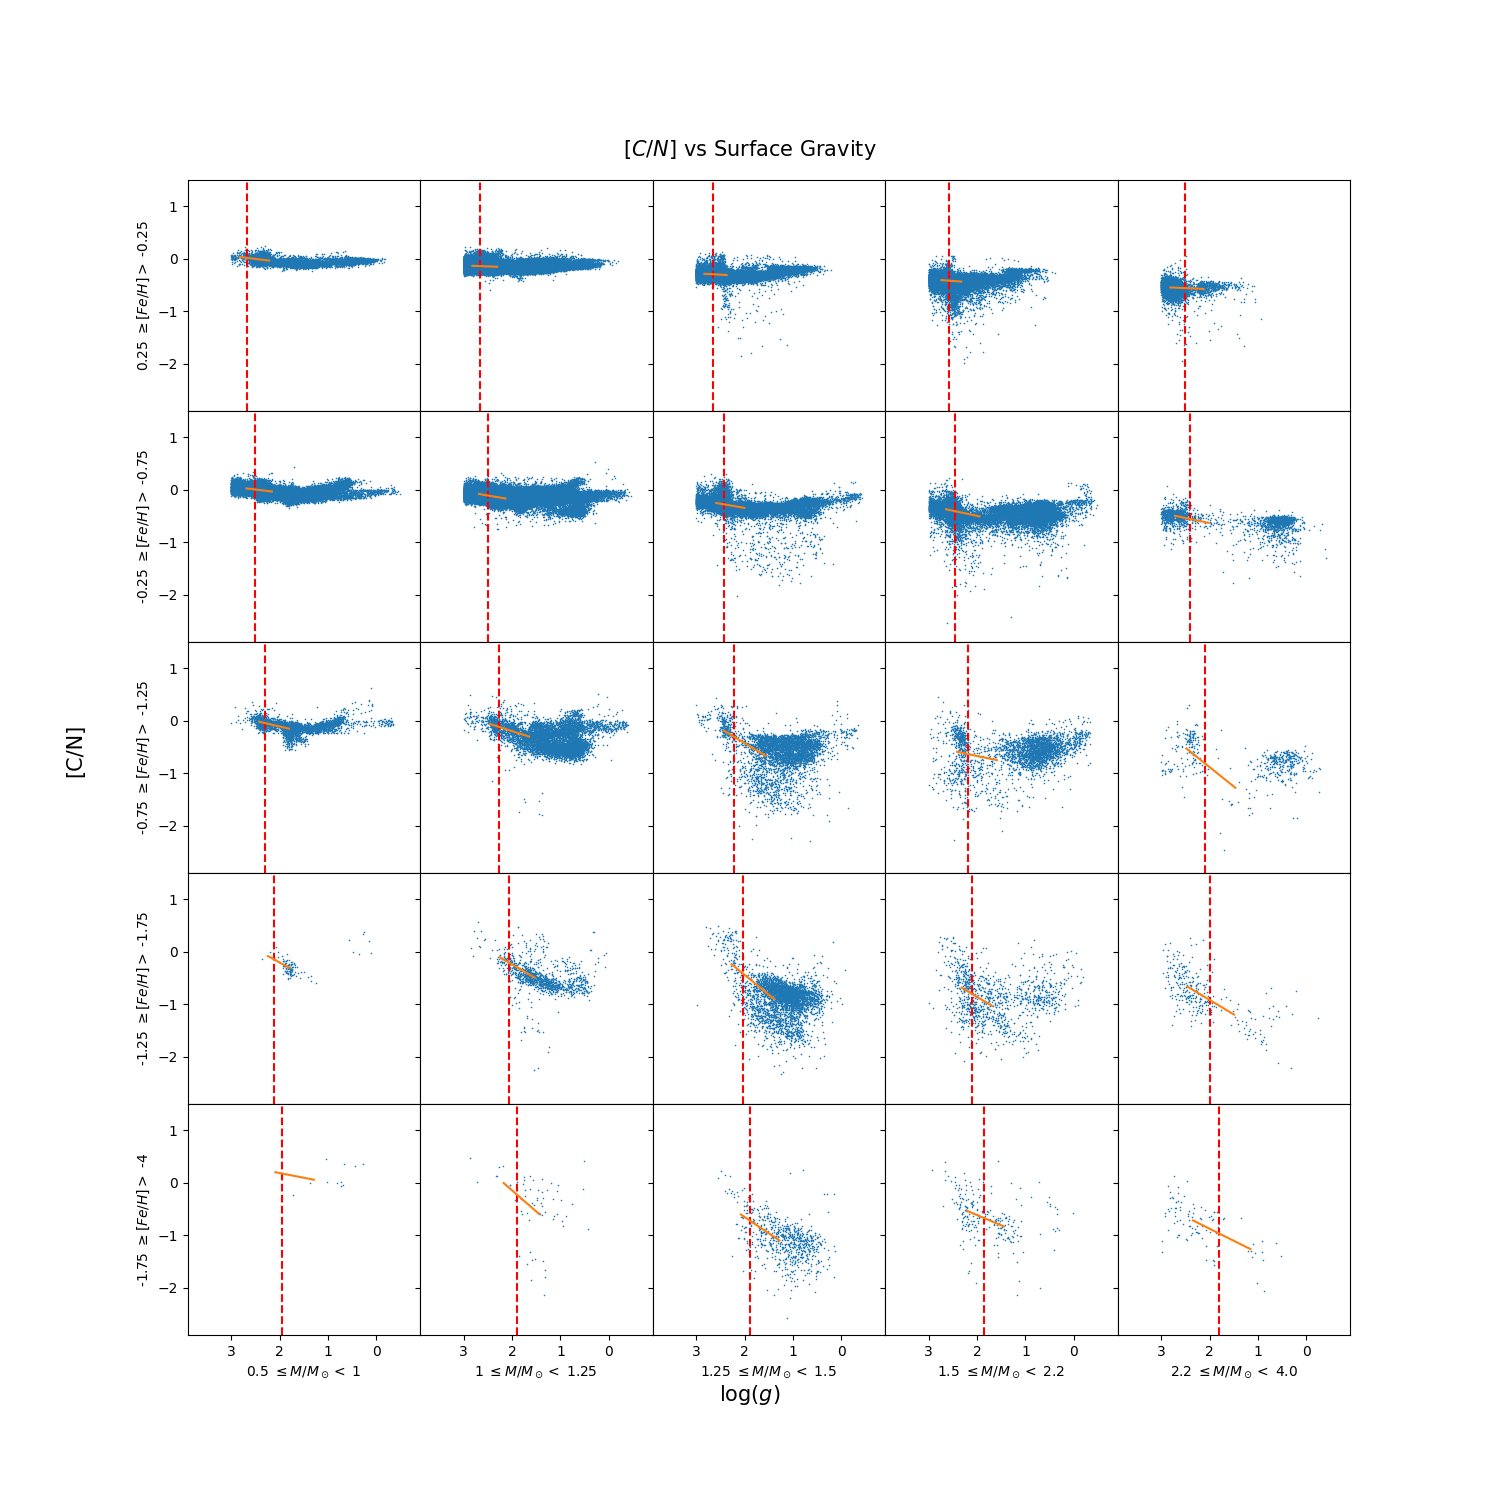
\includegraphics[width=.8\columnwidth]{Figures/DeepMixing.png}
\end{column}

\begin{column}{0.3\textwidth}
    The $\Big[\frac{C}{N}\Big]$ for stars, separated based on mass and metallicity. The vertical red line indicates where deep mixing theoretically begins. The orange lines show the change between average $\Big[\frac{C}{N}\Big]$ before and after deep mixing has theoretically begun
\end{column}
\end{columns}

\end{frame}
\subsection{Discussion}
\begin{frame}
\begin{columns}
   \begin{column}{0.5\textwidth}
        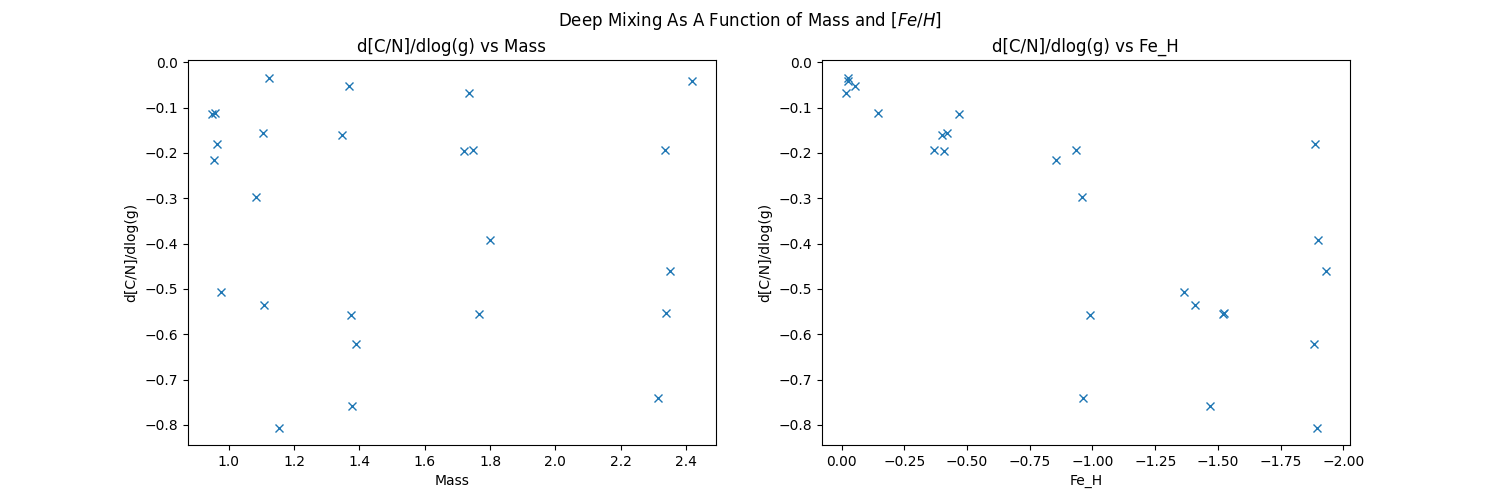
\includegraphics[width=1.2\columnwidth]{Figures/DeepMixingRate.png}
   \end{column}
\begin{column}{0.5\textwidth}
     
   \begin{itemize}
        \item As metallicity decreases, mixing rate increases (EXPECTED)
        \item As mass decreases, mixing rate does not increase (UNEXPECTED)
        \item Mixing occurs for stars with $M>2.2M_\odot$ (UNEXPECTED)
        \item Recovery in \CN for some stars (UNEXPECTED)
        \item Low \CN stars (UNEXPECTED)
   \end{itemize}
\end{column}
\end{columns}
\end{frame}


\begin{frame}
\begin{columns}
   \begin{column}{0.5\textwidth}
        \centering
        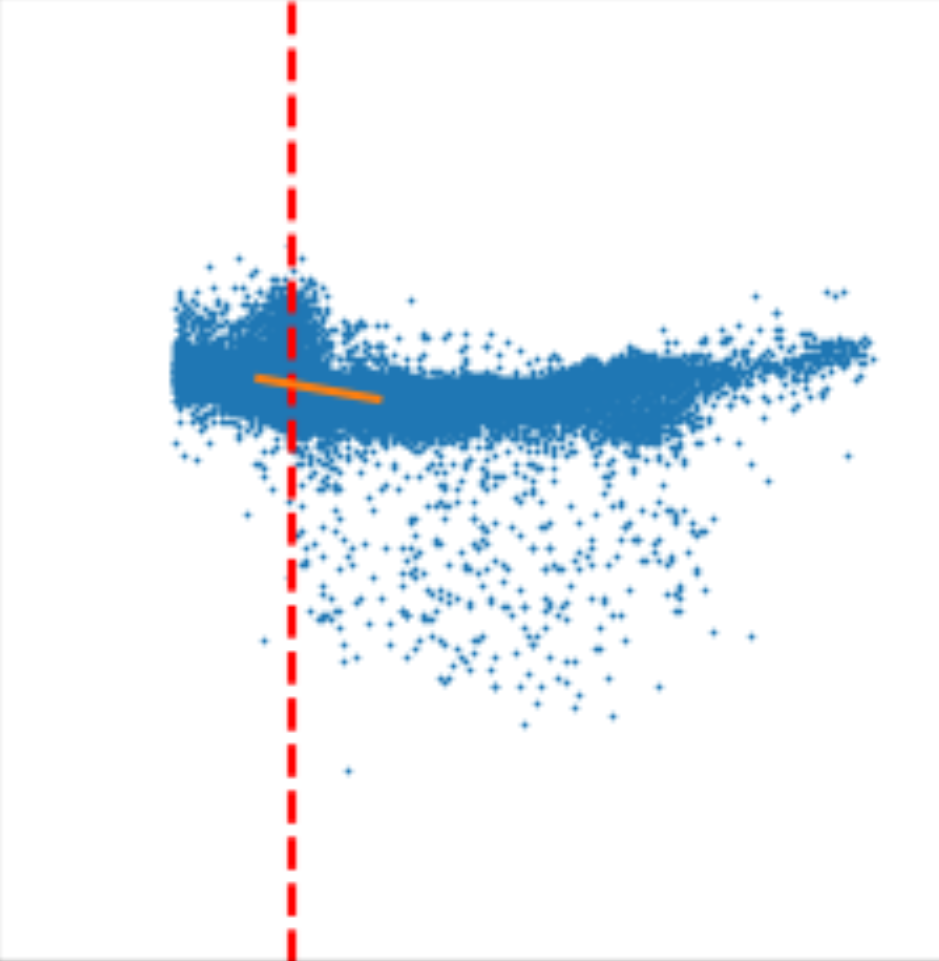
\includegraphics[width=.7\columnwidth]{Figures/Fe(-0.25,-0.75)Mass(1.25,1.5).png}
   \end{column}
\begin{column}{0.5\textwidth}
    The figure shows stars with \abundance{Fe}{H} between -0.25 and -0.75 and mass between 1.25\SM and 1.5\SM.
    \begin{itemize}
        \item We notice that towards the end of the graph (as $\log(g)$ decreases), the \CN has an upwards trend. Why?
        \item We can also notice that there are significant number of stars below the main group. Why?
    \end{itemize}
\end{column}
\end{columns}
\end{frame}


\subsubsection{Low \CN Stars}
\begin{frame}{Globular Clusters}
    \begin{columns}
      \begin{column}{0.7\textwidth}
            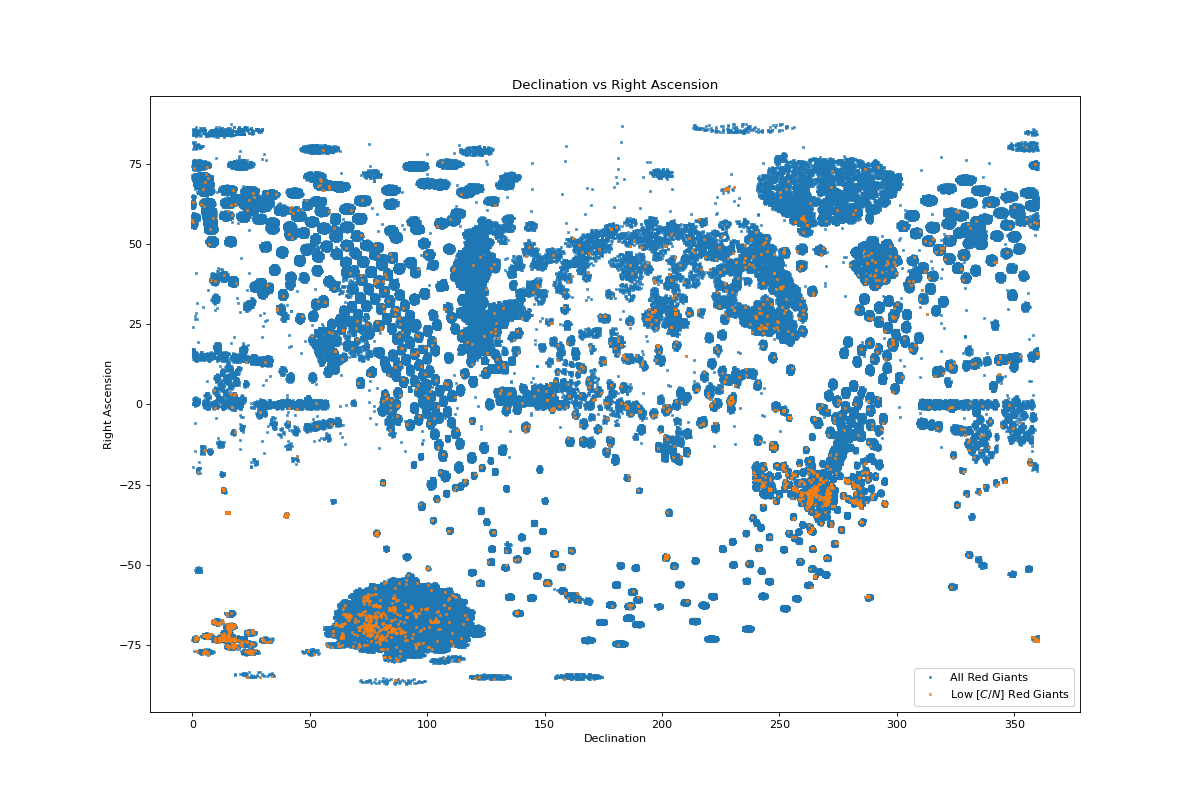
\includegraphics[width=\columnwidth]{Figures/PositionOfLowCNStars.png}
      \end{column}
      \begin{column}{0.4\textwidth}
            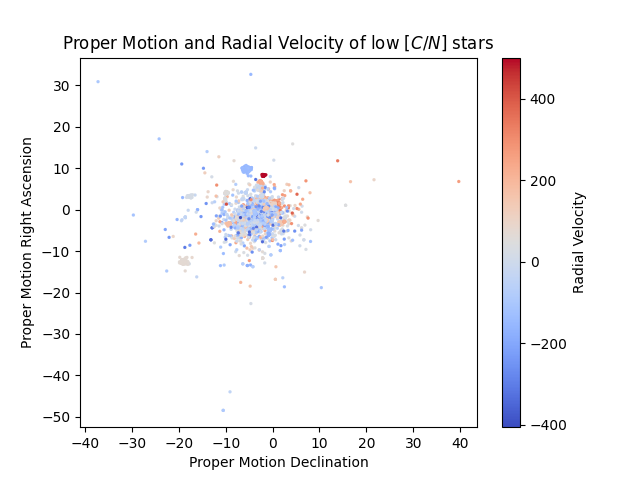
\includegraphics[width=\columnwidth]{Figures/LowCNStarsMotion.png}
      \end{column}
    \end{columns}
    \begin{center}
    Verdict: Globular Clusters do not explain all the low \CN stars.
    \end{center}
\end{frame}

\begin{frame}{Asymptotic Giant Branch (AGB) Stars}
    \begin{figure}
        \centering
        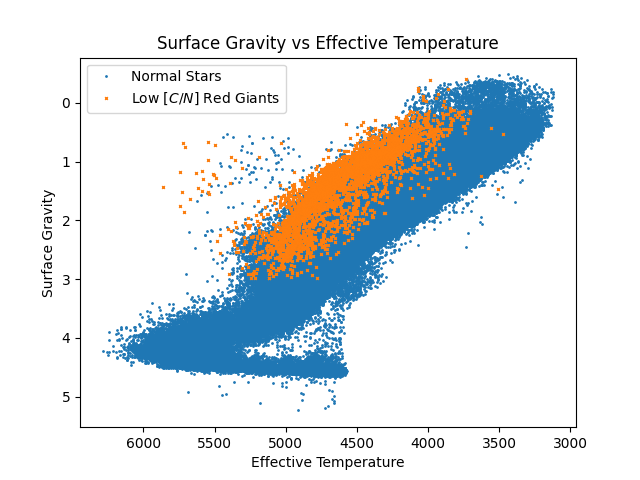
\includegraphics[width=0.5\columnwidth]{Figures/AGBProof.png}
    \end{figure}
    \begin{center}
        Verdict: AGB Stars do not explain all the low \CN stars.
    \end{center}
\end{frame}